\documentclass[11pt]{article}

\usepackage[pdftex]{graphicx} % OU
% \usepackage[dvips]{graphicx}

% \usepackage[round]{natbib}
\usepackage{adjustbox,array,url,hyperref,multirow,makecell,tabularx,caption,subcaption}
% \usepackage{url,hyperref,multirow,makecell}
\usepackage[table]{xcolor}
\usepackage{lipsum}
\usepackage{cite}
\usepackage{amsfonts}
%\usepackage[latin1]{inputenc}
\usepackage[utf8]{inputenc}
%\usepackage[brazilian,brazil]{babel}
%\usepackage{apacite}
%\usepackage{float}
\usepackage{booktabs}
\usepackage{multirow}

\usepackage{todonotes}
\newcommand{\pmendes}[1]{\color{blue}\textbf{paulo says: }#1\color{black}}

\usepackage{tikz}
\usetikzlibrary{
  angles,
  arrows,
  arrows.meta,
  calc,
  intersections,
  positioning,
  quotes,
  shapes.geometric,
  through,
}
\tikzset{
  x=0em,
  y=0em,
  node distance=1.2em,
  >=stealth',
}

\newcommand*\rot[1]{\rotatebox{90}{#1}}

\newtheorem{proposition}{Proposition}
\newtheorem{lemma}{Lemma}
\newtheorem{theorem}{Theorem}

\newcommand{\CQD}{\mbox{\rule[0pt]{1.5ex}{1.5ex}}\medskip}
\newcommand{\M}{\mathcal{M}}

\setlength{\oddsidemargin}{0.5cm} \setlength{\textwidth}{15cm}
\setlength{\topmargin}{-1.5cm} \setlength{\textheight}{22.3cm}%{24.7cm}

\usepackage{pdfpages}

\begin{document}

\LARGE

% \bigskip

%% TITLE
\begin{center}
{\bf Spatiotemporal Localization of Actors   in Video/360-Video and its Applications}
\end{center}


\bigskip
\normalsize

\begin{flushright}

Paulo Renato Conceição Mendes\\
Pontifical Catholic University of Rio de Janeiro\\
\texttt{paulo.mendes@telemidia.puc-rio.br}
\end{flushright}


\date{}

% $~$ \\

\thispagestyle{empty}

%
%%%% Abstract
\noindent {\bf Abstract.} 


% \medskip
\medskip

\noindent {\bf Keywords:}

\medskip
% \bigskip

% \newpage
\pagenumbering{roman} \setcounter{page}{-1}

% TABLE OF CONTENTS -  OPTIONAL
%\newpage
\tableofcontents

%% BEGIN DOCUMENT
\newpage
\pagenumbering{arabic} \setcounter{page}{1}


%%% Sections....
\section{Introduction}

The recent emergence of popular omnidirectional cameras and Head-Mounted-Displays (HMDs) has increased the amount of 360-video content available \cite{mendes_2020}. Omnidirectional videos are spherical visual signals that allow the viewer to look around a full 360-degree view of a scene from a specific point. When using HMDs, at each instant in time, the viewer is presented with a viewport that is updated as the viewer moves their head. This type of content, especially when consumed through Virtual Reality~(VR) devices (HMDs included), can provide immersive experiences in which the user has a strong feeling of presence when compared with the use of traditional media \cite{montagud_culture_2020}.

Several people use subtitles when consuming audiovisual media, and these subtitles are important in contributing to the understanding of the video content \cite{brown_subtitles_2017}. There are even people who choose to consume videos without the sound turned on \cite{hughes_disruptive_2019}. Additionally, the work of \citeonline{hayati2011effect}, as referenced in \citeonline{hughes_disruptive_2019}, shows that consumers are more likely to watch videos entirely if they have subtitles presented with them. In traditional 2D videos, static subtitles are commonly used and they are usually placed at the center-bottom of the screen \cite{rothe_dynamic_2018}.

Different from traditional 2D videos, subtitles positioning in 360-videos is challenging because it envolves both temporal and spatial domains \cite{agullo2019making}, and there is no ``center-bottom" of the screen in a 360-video \cite{brown_subtitles_2017}. Most current solutions rely on positioning subtitles either statically to the viewer or at fixed position in the 360-degree environment \cite{mendes_2020}. According to \citeonline{li_impacts_2018}, in a journalistic 360-videos case study, the subtitles viewing behaviour is dependent on the type of content. 

The remainder of this dissertation proposal is structured as follows. Section~\ref{sec:subtitles} presents the current solutions for subtitles positioning in 360º video. Section~\ref{sec:approach} details our approach for automatic subtitles positioning. Finally, Section~\ref{sec_4} presents some final considerations such as the current status of our work, the next steps, and the work schedule.
\section{Related Work}
\label{sec:related_work}

In this section we make a brief review of the works related to ours in the applications we intend to investigate in our dissertation.

\subsection{Video Face Recognition}

Face detection and recognition have been attracting the attention of researchers for more than two decades. Since the deep learning boom, face detection and recognition performance have greatly improved in terms of both speed and accuracy~\cite{masi2018deep}. Nowadays, face recognition systems are used for video surveillance and security systems, video analytics systems, smart shopping, automatic face tagging in photo collections, investigative tools that search for identities in social networks based on face images, and in thousands of other applications in our daily lives.

%Traditional deep learning models for face recognition such as DeepFace~\cite{taigman2014deepface} and DeepID~\cite{sun2014deep} use a CNN with fully-connected layer output to produce a representation of high-level features (face embeddings) from an input image, followed by a softmax layer to indicate the identity of classes. Other approaches, such as FaceNet~\cite{schroff2015facenet}, can directly measure the similarity among faces using euclidean space. Inspired by DeepID, this model uses the \textit{triplet loss} as the loss function to estimate similarity to one character's face to a  collection of other faces. Triplet loss improves the accuracy of the  CNN output by minimizing the euclidean distance between the anchor and the positive (face of the same identity) while maximizing the distance between the anchor and the negative (face of another identity). In this work, we evaluated different pre-trained CNN backbones on VGGFace2 dataset~\cite{cao2018vggface2} to generate the face embeddings. This model is the state-of-the-art\footnote{https://paperswithcode.com/paper/vggface2-a-dataset-for-recognising-faces} in the face verification task on the IJB-B dataset~\cite{whitelam2017iarpa}. 

%Proprietary systems for face recognition and matching are widely used by social network platforms. For instance, Facer~\cite{hazelwood2018applied} is Facebook's face detection and recognition framework. Given a photograph, it first detects all the faces. Then, it runs a  deep model to determine the likelihood of that face belonging to one of the top-N user friends. This allows  Facebook to suggest which friends the user might want to tag within the uploaded photographs. FindFace\footnote{https://findface.br.aptoide.com/app} is an app that matches photos to profile pictures on VKontakte,\footnote{https://vk.com/} a Russian social networking website similar to Facebook. FindFace uses a deep model developed by NTech Lab that won the \textit{2017 IARPA Face Recognition Prize Challenge} (FRPC)~\cite{grother20172017}  in two nominations out of three (“Identification Speed” and “Verification Accuracy”). Similarly, our method can detect faces in videos and automatically recognize their identities by a clustering-based algorithm that uses a knowledge base with the faces pre-identified as a reference; however, a comparison with such methods was not possible due to access restrictions.

Some recent works are focused on video face recognition. Pena \textit{et al.}~\cite{globofacestream} proposed a face recognition system to detect characters within videos, called~\textit{Globo Face Stream}. Their method uses a Histogram of Oriented Gradients (HOG) feature combined with a linear classifier to detect faces. Next, they use  FaceNet to generate the embeddings, followed by the euclidean distance calculus to measure the similarity among faces. Yang \textit{et al.}~\cite{yang2017neural} proposed a deep network for video face recognition called NAN (Neural Aggregation Network). They use a CNN to generate the embeddings, followed by an aggregation module that consists of two attention blocks which adaptively aggregate the feature vectors to form a single feature inside the convex hull spanned by them. Rao \textit{et al.}~\cite{rao2017attention} proposed a method for video face recognition based on attention-aware deep reinforcement learning. They formulated the process of finding the attention of videos as a Markov decision process and training the attention model without using extra labels. Unlike existing attention models, their method takes information from both the image space and the feature space as the input to make use of face information that is discarded in the feature learning process. Sohn \textit{et al.}~\cite{sohn2017unsupervised} proposed an adaptative deep learning framework for image-based face recognition and video-based face recognition. Given an embedding generated by a CNN, their framework adaptation is achieved by (1) distilling knowledge from the network to a video adaptation network through feature matching, (2) performing feature restoration through synthetic data augmentation, and (3) learning a domain-invariant feature through an adversarial domain discriminator. 

Like~\cite{globofacestream, yang2017neural, rao2017attention, sohn2017unsupervised}, our method uses a CNN to generate face embeddings from face images, with the difference that it uses an unsupervised cluster-based method to compare the similarity among face datasets and faces extracted from videos. Also, our approach can detect faces that do not have an identity registered in the face dataset with excellent performance.

\subsection{Educational Video Recommendation}

Regarding \textit{Educational Video Recommendation}, we cite works based on content-filtering.
These works perform analyses and comparisons using the video textual description or speech recognition performed on them. 
Omisore \textit{et. al.} \cite{omisore2014personalized}, for example, propose combining \textit{fuzzy} techniques to recommend books with content suitable for students based on their reading histories in a digital library, while Mahajan \textit{et. al.} \cite{mahajan2015optimising} propose, given a reference video,  mining social media, and web for suggesting links for a student to visit.
Moreover, Barrére \textit{et. al.}
~\cite{barrere2020utilizaccao} use texts from speech recognition to create recommendations.
These works are only based on textual characteristics~(or content converted to it) for performing recommendations.
Our work focuses on using a visual part of the video, more precisely the presence of actors.

\subsection{Subtitles Positioning in 360-video}
\label{sec:subtitles}

Some works have proposed solutions for subtitles positioning based on the current viewport of the user.
%%
When defining the \emph{static-follow} strategy, \citeonline{brown_subtitles_2017} argue that it is a common behaviour for showing information in Virtual Reality~(VR) experiencies, as part of a ``head-up display'' (HUD). In this strategy, the subtitles are shown to the viewer as if they were static relative to their head, by following the viewer as they look around the environment. 
%%
The work of \citeonline{brown_subtitles_2017} define the \emph{lag-follow} stategy to address the sickness related to the \emph{static-follow} strategy while still keeping the subtitles visible to the viewer. Similar to the \emph{static-follow} strategy, the subtiles appear in front of the viewer. It remains in such posititon~(relative to the environment) until the viewer's head rotates more than the 30º threshold. The subtitles then smoothly rotates to be in front of the viewer again. 


Other works investigate the usage of subtitles positioned relatively to the world.
%%
In the \emph{Repeated Subtitles} strategy~\cite{brown_subtitles_2017}, repeated subtitles are placed around the user. These subtitles stay fixed in the environment and do not follow the user's head motion.
%%
In the \emph{Appear} strategy~\cite{brown_subtitles_2017}, the subtitles are placed at the centre of the user's field of view horizontally, 15º bellow eye-level. If the viewer moves their head, the subtitles remain static within the environment and do not follow their gaze. 

More recently, some works have used more complex solutions.
%%
As referring to annotations~(that could be subtitles), \citeonline{matos_dynamic_2018} say that there are cases where the point of interest is moving through the video, which requires a dynamic annotation that follows its movement. 
%%
In the \emph{speaker-following subtitles} strategy~\cite{rothe_dynamic_2018}, the subtitles are placed close to the speaker. 
%%
Similar to the work of \citeonline{rothe_dynamic_2018}, we intend to position subtitles close to the speakers in the 360-video. The main difference of our work, however, is that we automatically detect the actors present in a 360-video and use their position for placing the subtitles according to an authoring model we propose.
  


\section{Video Face Clustering}
\label{sec:video_face_clustering}

\begin{figure*}[!ht]
    \centering
    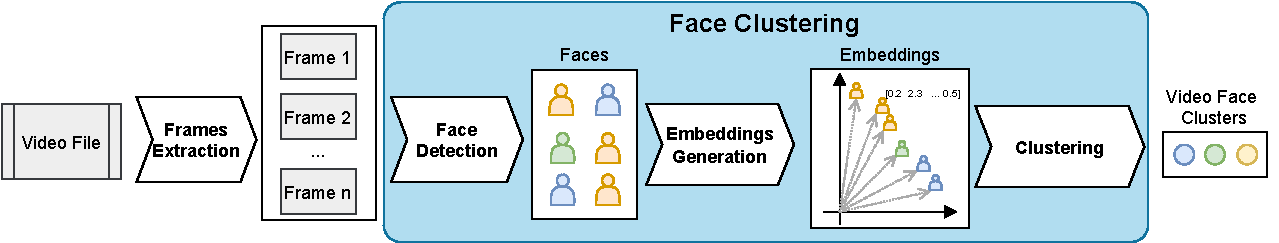
\includegraphics[width=\textwidth]{img/video_face_clustering.pdf}
    \caption{Video face clustering process.}
    \label{fig:video_face_clustering}
\end{figure*}

The core of this dissertation is a method that we call \emph{Video Face Clustering}.
%%
It consists in detecting and grouping faces from different video frames~(ideally from the same actors) extracted from a video file.
%%
Figure \ref{fig:video_face_clustering} depicts this process.
%%
Each of its steps are described in the next paragraphs.


First, we perform \textit{Frames Extraction} by receiving a video file as input and extracting its frames according to a given frame rate. 

The \textit{Face Detection} step uses an object detection model for detecting faces in each of its images.
%%
This model is responsible for returning the bounding boxes of the faces present in the image, specified by the $x$ and $y$ axes coordinates of the upper-left corner and of the lower-right corner of the rectangle that establishes the visual limits that encapsulate each face. 
%%
With these bounding boxes, we can isolate and extract the bounded images, obtaining a dataset composed of images of faces only.

The \textit{Face Detection} step uses an object detection model for detecting faces in each of its images.
%%
This model is responsible for returning the bounding boxes of the faces present in the image, specified by the $x$ and $y$ axes coordinates of the upper-left corner and of the lower-right corner of the rectangle that establishes the visual limits that encapsulate each face. 
%%
With these bounding boxes, we can isolate and extract the bounded images, obtaining a dataset composed of images of faces only.


The objective of the \textit{Embeddings Generation} step is to represent each face image as a vector space in $\mathbb{R}^{n}$.
%%
To achieve that, it processes each of the faces generated in the previous step through a CNN, generating embeddings. 
%%
An embedding is a representation of the input in a lower dimensional space.

In the \textit{Clustering} step, we group embeddings and, consequently, faces that are close in the embedding space using a clustering algorithm. 
%%
The clustering process should produce a partition of the dataset, i.e., each generated cluster represents a specific person, and the union of all clusters covers the whole dataset.

By the end of this process, we expect to have the spatiotemporal localization of the actors present in a video file.
%%
Figure \ref{fig:timeline} shows an example of the results achieved by this method. It contains a timeline of a video with lines coloring the segments that each actor appears.

\begin{figure}[!ht]
    \centering
    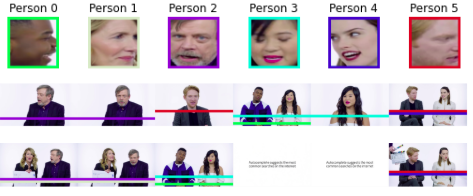
\includegraphics[width=0.6\linewidth]{img/webmedia/timeline2.png}
    \caption{Timeline with tagged frames by their clusters}
    \label{fig:timeline}
\end{figure}

We have evaluated this process by the quality of the clusters generated with different combinations of Convolutional Neural Networks (CNNs) and clustering algorithms. Details about this evaluation will be presented in our dissertation. 


\section{Applications}
\label{sec:applications}

This section describes the applications we intend to investigate in our dissertation. 
%%
These three applications propose novel approaches for tasks in video using spatiotemporal localization of actors through \emph{video face clustering}.



\subsection{Cluster-Matching-Based Method For Video Face Recognition}
\label{webmedia}

In this first application, we propose a cluster-matching-based approach for video face recognition where \emph{face clustering} is used to group faces in both the face dataset and in the target video~(video face clustering).
%%
Consequently, classes do not have to be previously known, and the effort spent with annotations is significantly reduced --- as it is done over clusters instead of single images.
%%
Face recognition becomes a task of comparing clusters from the dataset with the ones extracted from images or video sources.
%%
Therefore, our approach is easily scalable.

In our approach we use \emph{face clustering} in an images dataset and in the referenced video. Then, the clusters of the images dataset are labeled. Next, we perform \emph{Cluster Matching} where the clusters from the image dataset and from the video are matched using a heuristic based on clusters distance. Figure \ref{fig:cluster_matching} shows our proposed approach.


\begin{figure*}[!ht]
    \centering
    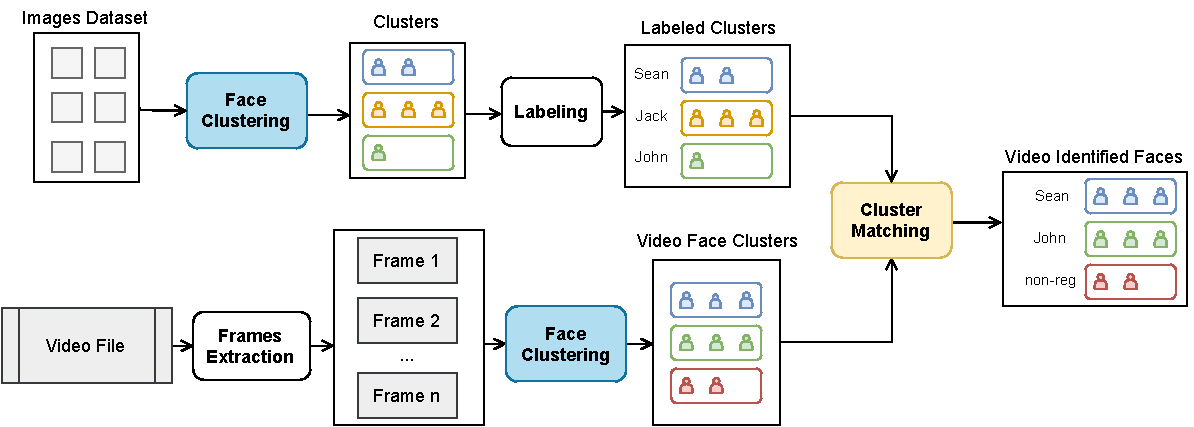
\includegraphics[width=\textwidth]{img/webmedia/cluster_matching_process.pdf}
    \caption{Cluster-Matching based Method for Video Face Recognition.}
    \label{fig:cluster_matching}
\end{figure*}

We have performed two experiments to evaluate our method. 
%%
The first evaluation aimed at measuring how well our approach of \emph{Cluster Matching} performed when clustering images of actors in different occasions~(instead of frames from a video). 
%%
The second evaluation aimed at measuring how well our approach performed on video. Each of these evaluations will be described in details in our dissertation. This application has also been published at a relevant multimedia conference~\cite{mendes2020cluster}.
%%
Figure \ref{fig:timeline_pol} shows an example of our method for video face recognition in a video where two identified Brazilian politicians are shown in each frame with its respective colored cluster.

\begin{figure}[!ht]
    \centering
    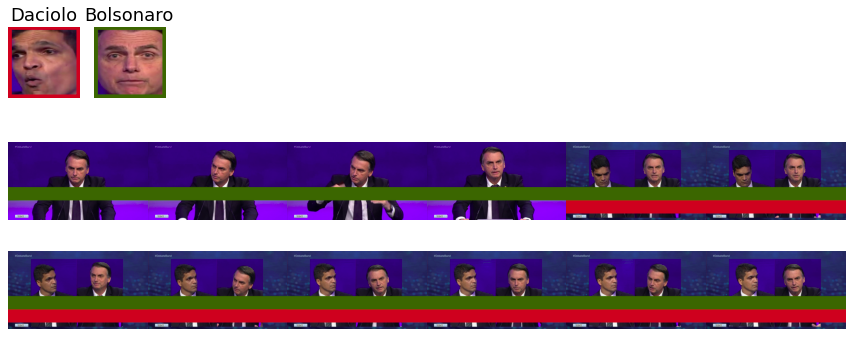
\includegraphics[width=0.6\linewidth]{img/webmedia/timeline_pol.png}
\vspace{-1em}
    \caption{Timeline with tagged frames by their clusters of registered people}
    \label{fig:timeline_pol}
\end{figure}



\subsection{A Clustering-Based Method for Automatic Educational Video Recommendation Using Deep Face-Features of Actors}

In this second application we used \emph{video face clustering} for recommending videos that share the presence of the same actors. %%
This work aimed at recommending educational video content based on actors' presence.
%%
To do that, we perform \emph{video face clustering} in all videos from a certain dataset and calculate their centroids.
%%
By the end of this step, we have each video in the dataset represented by its centroids where, ideally, each centroid represents an actor present in the video.


Given these centroids, we perform a clustering step for creating a relationship between videos that share the presence of the same actors.
%%
By doing that, we group centroids from the same actor that are in different videos. For instance, in Figure \ref{fig:video_recommendation}, one can see that the \emph{purple actor} is present in both Videos 1 and 2, while the \emph{orange actor} is present in both Videos 2 and n. 
%%
By the end of this step, we have the group $L$ of actors present in the dataset of videos $V$, and we can also denote $L_v$ as the group of actors present in video $v$.

\begin{figure*}[!ht]
  \centering
  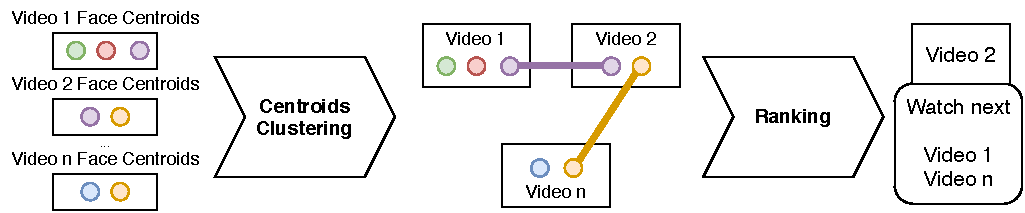
\includegraphics[width=0.8\linewidth]{img/ism/video_recommendation.pdf}
  \caption{Video Recommendation process.}
  \label{fig:video_recommendation}
\end{figure*}

Finally, we rank the recommended videos based on the amount of time the referenced actors were present.
%%
For doing that, we compute a similarity score using the presence of the actors in the current video and the presence of these same actors in the other video.
%%
Let $p_{l,v}$ denote the percentage of frames in which the actor $l \in L_v$ is present in video $v \in V$. For each video $v \in V$ and $u \in V-v$ we compute a score of similarity $S_{v,u}$.

\vspace{-1em}
\begin{equation}
  S_{v,u} = \sum_{l~\in~L_v}{p_{l,v}\cdot{p_{l,u}}}
\end{equation}

Using this score for each video $v$ we compute a ranking $R_{v}$ where $R_{v,i}$ denotes the \emph{i-greatest} $S_v$ and $R_{v,i}\ge~R_{v,i+1}$ for all $i~\in~1...n_v$, where $n_v$ is the number of videos $u$ in which $S_{v,u}>~0$. 
%%
In this way, the more actors a video have in common with the reference video, and the more time these actors are present in both videos, the higher the video is positioned in the ranking of the reference video.  
%%
By the end of this pipeline, we have a ranking of recommended videos for each video in the dataset.
%%
It is important to notice that our method is unsupervised and does not require the information of the actors in advance.
%%
Consequently, we do not store any information regarding the identity of the actors, respecting their privacy.
%%
A particular feature of this approach is that it can be done without supervision, allowing for new videos to be automatically analyzed

We evaluate our approach based on the relevance of the videos recommended. 
%%
In our evaluation, we constructed a dataset of educational videos extracted from YouTube.
%%
Details about this evaluation will be described in our dissertation. 
%%
This application has also been published at a relevant multimedia conference~\cite{mendes2020ISM}.
\subsection{Automatic Subtitles Positioning in 360-Video}

In \cite{mendes2020authoring}, we proposed a model for authoring interactive 360° video. In such a model, we can define interactive 360° video that are presented together with additional information attached to it, such as image, text and spatial audio. The positioning of such additional information is defined by their polar coordinates, start time and duration. Moreover, we can also configure behaviours depending on where the user is looking. For instance, we can define that a text moves with the user's head motion and is always visible or that such text is placed at fixed position if it is in the field of view of the user. Besides the design of such a model, we developed a player that follows the definitions of our model and is able to play interactive 360° video defined by it. Then, we can use \emph{video face clustering} to define the positioning of subtitles according to the actors positioning using our player.

Nowadays, the most common way for representing and transmitting 360-video is using an equirectangular projection~\cite{yang2018object}. With the equirectangular projection, each sphere point is defined by two angles~\cite{snyder1987map}: \emph{latitude}~$\theta \in [-90^{\circ}, +90^{\circ}]$ and \emph{longitude}~$\phi \in [-180^{\circ}, +180^{\circ}]$. This kind of projection creates challenges for image processing and computer vision algorithms, especially to the convolution-based ones because of the severe distortions in areas vertically distant from the center of the image~(see Figure \ref{fig:equirectangular_proj}). Due to these distortions, we adapted the steps of our methods that use traditional CNNs: \emph{Face Detection} and \emph{Embeddings Generation}.

\begin{figure}[!ht]
\centering
    \begin{subfigure}{0.47\linewidth}
        \centering
        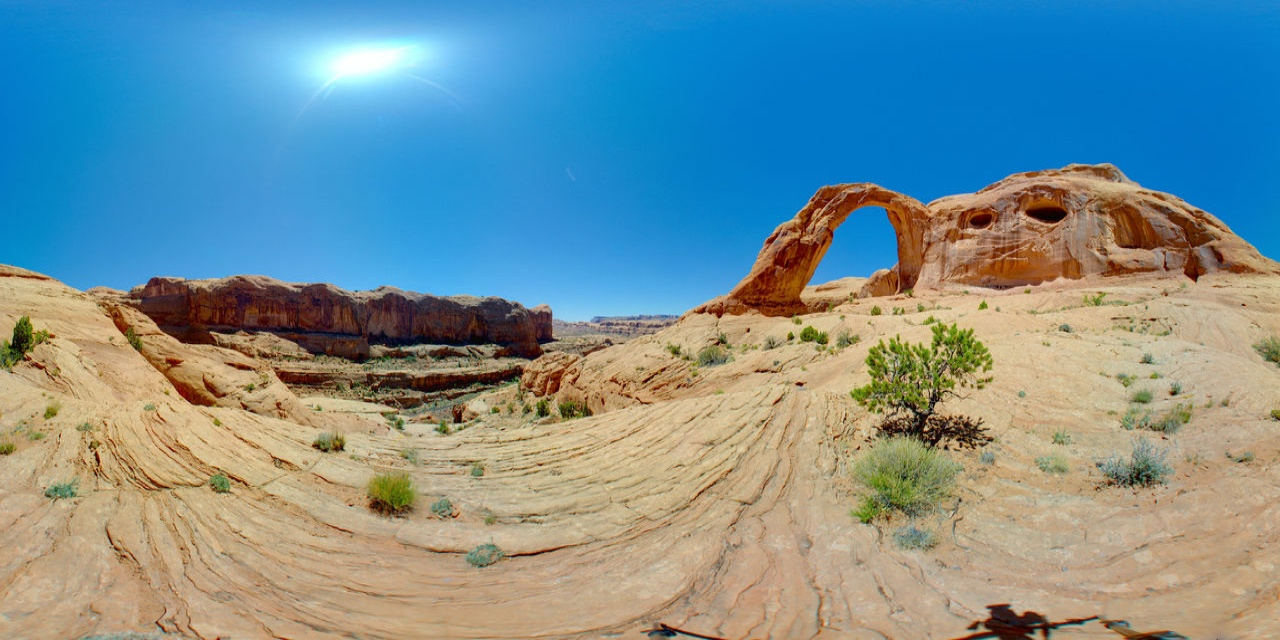
\includegraphics[width=1\textwidth]{img/image (9).jpg}
        \caption{Outdoor equirectangular image.}
        \label{subfig:out_equi}
    \end{subfigure}\hfill
    \begin{subfigure}{0.47\linewidth}
        \centering
        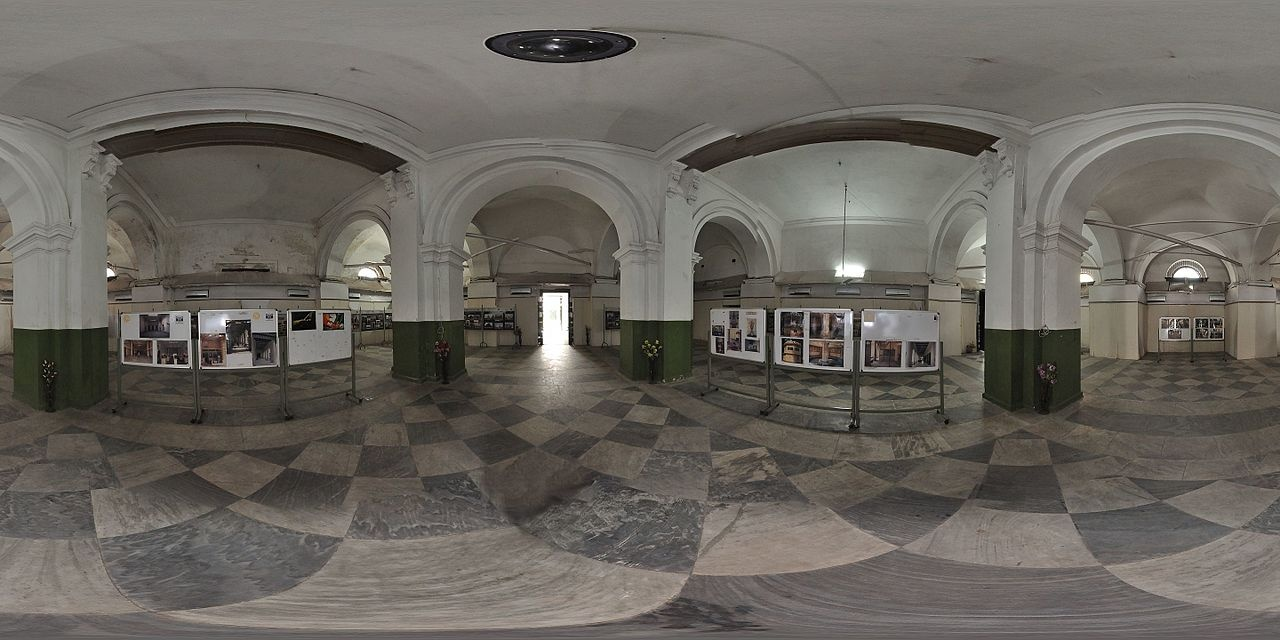
\includegraphics[width=1\textwidth]{img/image (10).JPG}
        \caption{Indoor equirectangular image.}
        \label{subfig:in_equi}
    \end{subfigure}

\caption{Examples of 360-images represented through equirectangular projection.}
\label{fig:equirectangular_proj}
\end{figure}




Because of the distortions present on the equirectangular projection, we opted for elaborating a solution based on viewports extraction. A viewport is defined by its center, in polar coordinates~(lat, long), and its field of view~(FoV). Figure \ref{fig:viewports} shows viewports extracted at different polar coordinates from Figure \ref{subfig:out_equi}.
%%
\begin{figure}[!ht]
    \centering
    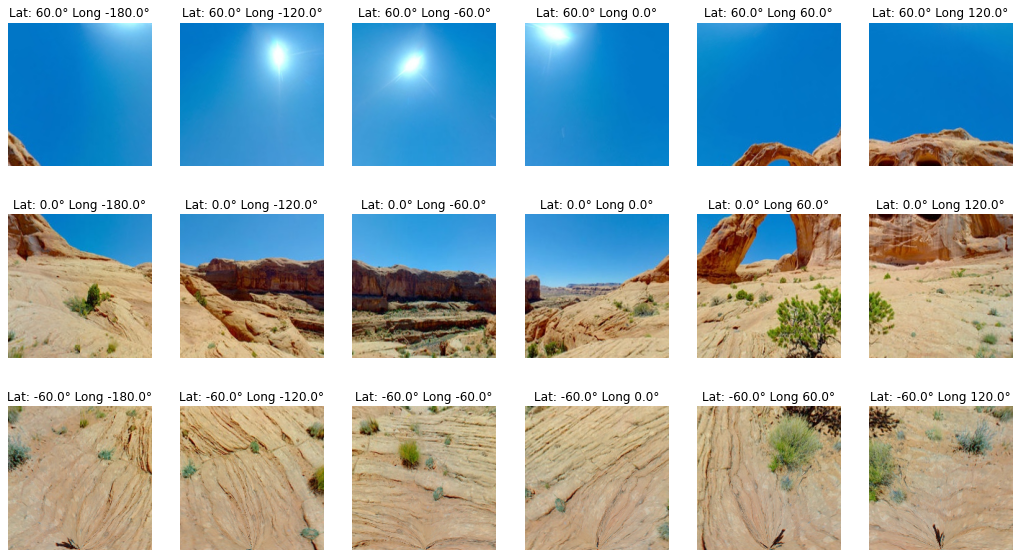
\includegraphics[width=1\textwidth]{img/viewports.png}
    \caption{Viewports extracted at different polar coordinates with $FoV = 60^{\circ}$}
    \label{fig:viewports}
\end{figure}
%%
For each viewport, we apply a face detection model. 
Then, we project the faces detected bounding boxes back to the equirectangular image. 
%%
After eliminating repeated detections with NMS, we perform \emph{Embeddings Generation} using the faces detected in the viewports~(with reduced distortions) instead of using its equivalent in the original equirectangular video frame.

By using these adaptations to the 360-video domain, we are able to apply \emph{video face clustering} to them and obtain the spatiotemporal localization of actors. With this in hands, we can automatically position subtitles close to the actors in the 360-video using our authoring model (see Figure \ref{subfig:subtitles_actor}). Moreover, as our authoring model supports interactivity, we can detect whether actors are in the FOV of the user. We can use this information to place subtitles in the bottom of the user's FOV when the actor speaking is not visible to the user. Thus, the subtitles are always visible to the user.


\begin{figure}[!ht]
\centering
    \begin{subfigure}{0.47\linewidth}
        \centering
        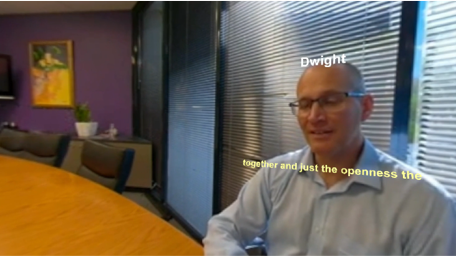
\includegraphics[width=1\textwidth]{img/video360/subtitles_actor.png}
        \caption{Subtitles positioning close to actors' face when they are in the user's FOV.}
        \label{subfig:subtitles_actor}
    \end{subfigure}\hfill
    \begin{subfigure}{0.47\linewidth}
        \centering
        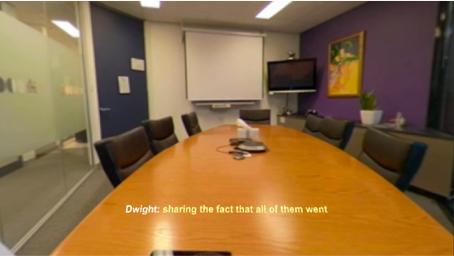
\includegraphics[width=1\textwidth]{img/video360/subtitles_bottom.png}
        \caption{Subtitles positioning in the bottom of user's FOV.}
        \label{subfig:subtitles_bottom}
    \end{subfigure}

\caption{Subtitles positioning using video face clustering and our authoring model.}
\label{fig:subtitles}
\end{figure}

Regarding this application, we point out the following remaining task:

\begin{itemize}
    \item T1 - Organize and tabulate evaluation results of face detection in equirectangular images.
\end{itemize}

\section{Contributions}
\label{sec_contritutions}
 As collateral contributions of this research, three papers have been published in relevant multimedia conferences \cite{mendes2020cluster, mendes2020authoring, mendes2020ISM}. In \cite{mendes2020authoring}, we have developed an authoring model and a player for interactive 360º video, enabling subtitles positioning. In \cite{mendes2020cluster}, we have evaluated video face clustering together with a cluster-matching method for video face recognition. In \cite{mendes2020ISM}, we have used video face clustering and the presence of actors in different video as a mean for recommending educational videos.
 
\section{Expected Contributions}
\label{sec_expected}
In our dissertation, we aim at exploring the usage of spatiotemporal localization of actors and its applications in video. We intend to investigate its usage in the tasks of video face recognition and educational video recommendation. Moreover, we will examine the applicability of this method in the authoring process of interactive 360-video with dynamic subtitles based on actors localization.


\section{Schedule}
\label{sec_schedule}
Table \ref{tab:schedule} presents the schedule we propose for completing the remainder tasks of this research.

\definecolor{darkgray}{RGB}{180,180,180}
\definecolor{gray}{RGB}{205,205,205}
\definecolor{lightgray}{RGB}{218,218,218}
\definecolor{lightlightgray}{RGB}{238,238,238}

\definecolor{darkred}{RGB}{204,0,0}
\definecolor{red}{RGB}{224,102,102}
\definecolor{lightred}{RGB}{244,199,195}

\definecolor{darkmagenta}{RGB}{61,133,198}
\definecolor{magenta}{RGB}{111,168,220}
\definecolor{lightmagenta}{RGB}{166,206,242}

% \definecolor{mark}{RGB}{224,102,102} %red
\definecolor{mark}{RGB}{111,168,220} %magenta

\definecolor{white}{RGB}{255,255,255}

\arrayrulecolor{white}
% \arrayrulecolor{darkgray}
\setlength\tabcolsep{3.0pt} % space between the text and the left/right border. Default Value = 6.0pt

\begin{table} [!ht]
  \centering
  \caption{Schedule of this dissertation proposal.}
  \label{tab:schedule}

  \begin{tabularx}{21em}{|p{6em}|p{5em}|p{5em}|p{5em}}
 
  \rowcolor{darkgray} & 
  \multicolumn{3}{|c|}{\textbf{2021}}\\ 
  
  \rowcolor{gray}
  \multicolumn{1}{|c|}{\multirow{-2}{*}{\cellcolor{darkgray}\textbf{Tasks}}} & 
  \multicolumn{1}{|c|}{\textbf{May}} & 
  \multicolumn{1}{|c|}{\textbf{Jun}} & 
  \multicolumn{1}{|c|}{\textbf{Jul}}\\
%   \hline
%%%%%%%%%%%%%%%%%%%%%%%%%%%%%%%%%%%%%%%%%%%%%%%%%%%%%%%%%%%%%%%%%%%%%%%%%%%%%%%%%%%%%%%%%%%%%%%%%%%%%%%%%%%%%%%%%%%%%%%%%%%%%%%%%%%%%%
  \rowcolor{lightgray}
       & \cellcolor{mark} &  &\\
  \rowcolor{lightgray}
    \multicolumn{1}{|c|}{\multirow{-1}{*}{T1}}
       & \cellcolor{mark} & &\\
  \rowcolor{lightgray}  
   & \cellcolor{mark} & & \\
%   \hline
%%%%%%%%%%%%%%%%%%%%%%%%%%%%%%%%%%%%%%%%%%%%%%%%%%%%%%%%%%%%%%%%%%%%%%%%%%%%%%%%%%%%%%%%%%%%%%%%%%%%%%%%%%%%%%%%%%%%%%%%%%%%%%%%%%%%%%
  \rowcolor{lightlightgray}
  &  & \cellcolor{mark}  & \cellcolor{mark}\\
  \rowcolor{lightlightgray}
    \multirow{-2}{*}{Dissertation} 
    &  & \cellcolor{mark}  & \cellcolor{mark}\\
  \rowcolor{lightlightgray}
    \multirow{-2}{*}{Writing} 
    &  & \cellcolor{mark}  & \cellcolor{mark}\\
%   \hline
%%%%%%%%%%%%%%%%%%%%%%%%%%%%%%%%%%%%%%%%%%%%%%%%%%%%%%%%%%%%%%%%%%%%%%%%%%%%%%%%%%%%%%%%%%%%%%%%%%%%%%%%%%%%%%%%%%%%%%%%%%%%%%%%%%%%%%
  \rowcolor{lightgray}
  &  &  & \cellcolor{mark}\\
  \rowcolor{lightgray}
    \multirow{-2}{*}{Dissertation} 
  &  &  & \cellcolor{mark}\\
  \rowcolor{lightgray}
  \multirow{-2}{*}{Presentation}
  &  &  & \cellcolor{mark}\\
\arrayrulecolor{darkgray}    

%   \end{tabular}
  \end{tabularx}
\end{table}

% Development of model instantiation
% Preliminary evaluation 
% Evaluation 
% Evaluation data analysis
% Thesis writing
% Thesis defense

\newpage
% \addcontentsline{toc}{section}{Referências}
\addcontentsline{toc}{section}{References}

\bibliographystyle{sbc}
% \bibliographystyle{plainnat}
\bibliography{sbc-template}

\end{document}
